This section presents an overview of the LEG processor, including the instruction set and memory architecture.
LEG has a five stage pipeline with Fetch, Decode, Execute, Memory, and Writeback stages.
Most control logic is implemented in the decode stage, and conditional execution is checked in the execute stage.

\subsection{Instruction Set}
\begin{figure}[h!]
\centering
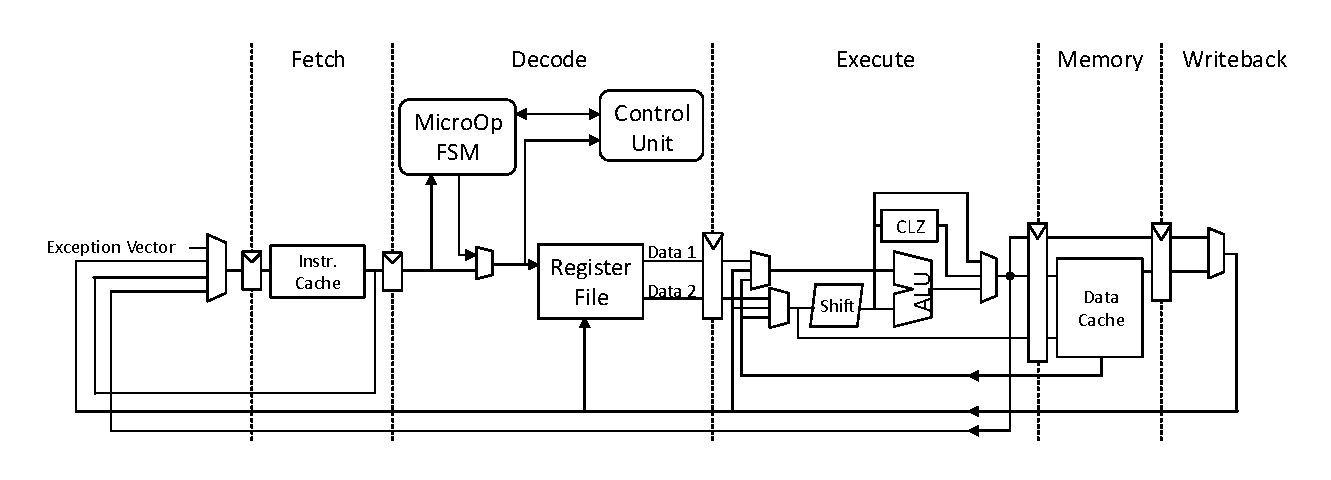
\includegraphics[width=\textwidth]{./diagrams/datapath_simple.pdf}
\caption{LEG processor core overview. More detailed diagrams are shown in the relevant sections below.}
\label{fig:core}
\end{figure}


LEG supports a subset of the ARMv5 instruction set. 
Known exceptions are the entire Thumb instruction set, LDM(2), and the rotate functionality of memory instructions.
The rotate functionality is not implemented because it appears to be unsupported in the version of qemu used to debug LEG.
All other addressing modes and instructions are supported, and any bugs that are discovered can be reported to the corresponding authors listed on the first page of this document.

The processor core is split into three main components.
The datapath contains the register file and hardware to execute arithmetic and memory operations, the controller sets multiplexers and other datapath control signals to create the specific behavior of each instruction, and the hazard unit detects dependencies between instructions and stalls the pipeline to resolve them.
A simplified overview of the processor core is summarized in Figure \ref{fig:core}.
More information about these subsystems can be found in later sections.
The datapath is described in Section \ref{sec:dp}, the controller in Section \ref{sec:c} and the hazard unit in Section \ref{sec:h}.

The full processor core diagram is shown in Figure \ref{fig:pipelinedfull} and is also included as a high quality PDF in the \texttt{documentation/diagrams} directory.

\begin{figure}[h!]
\centering
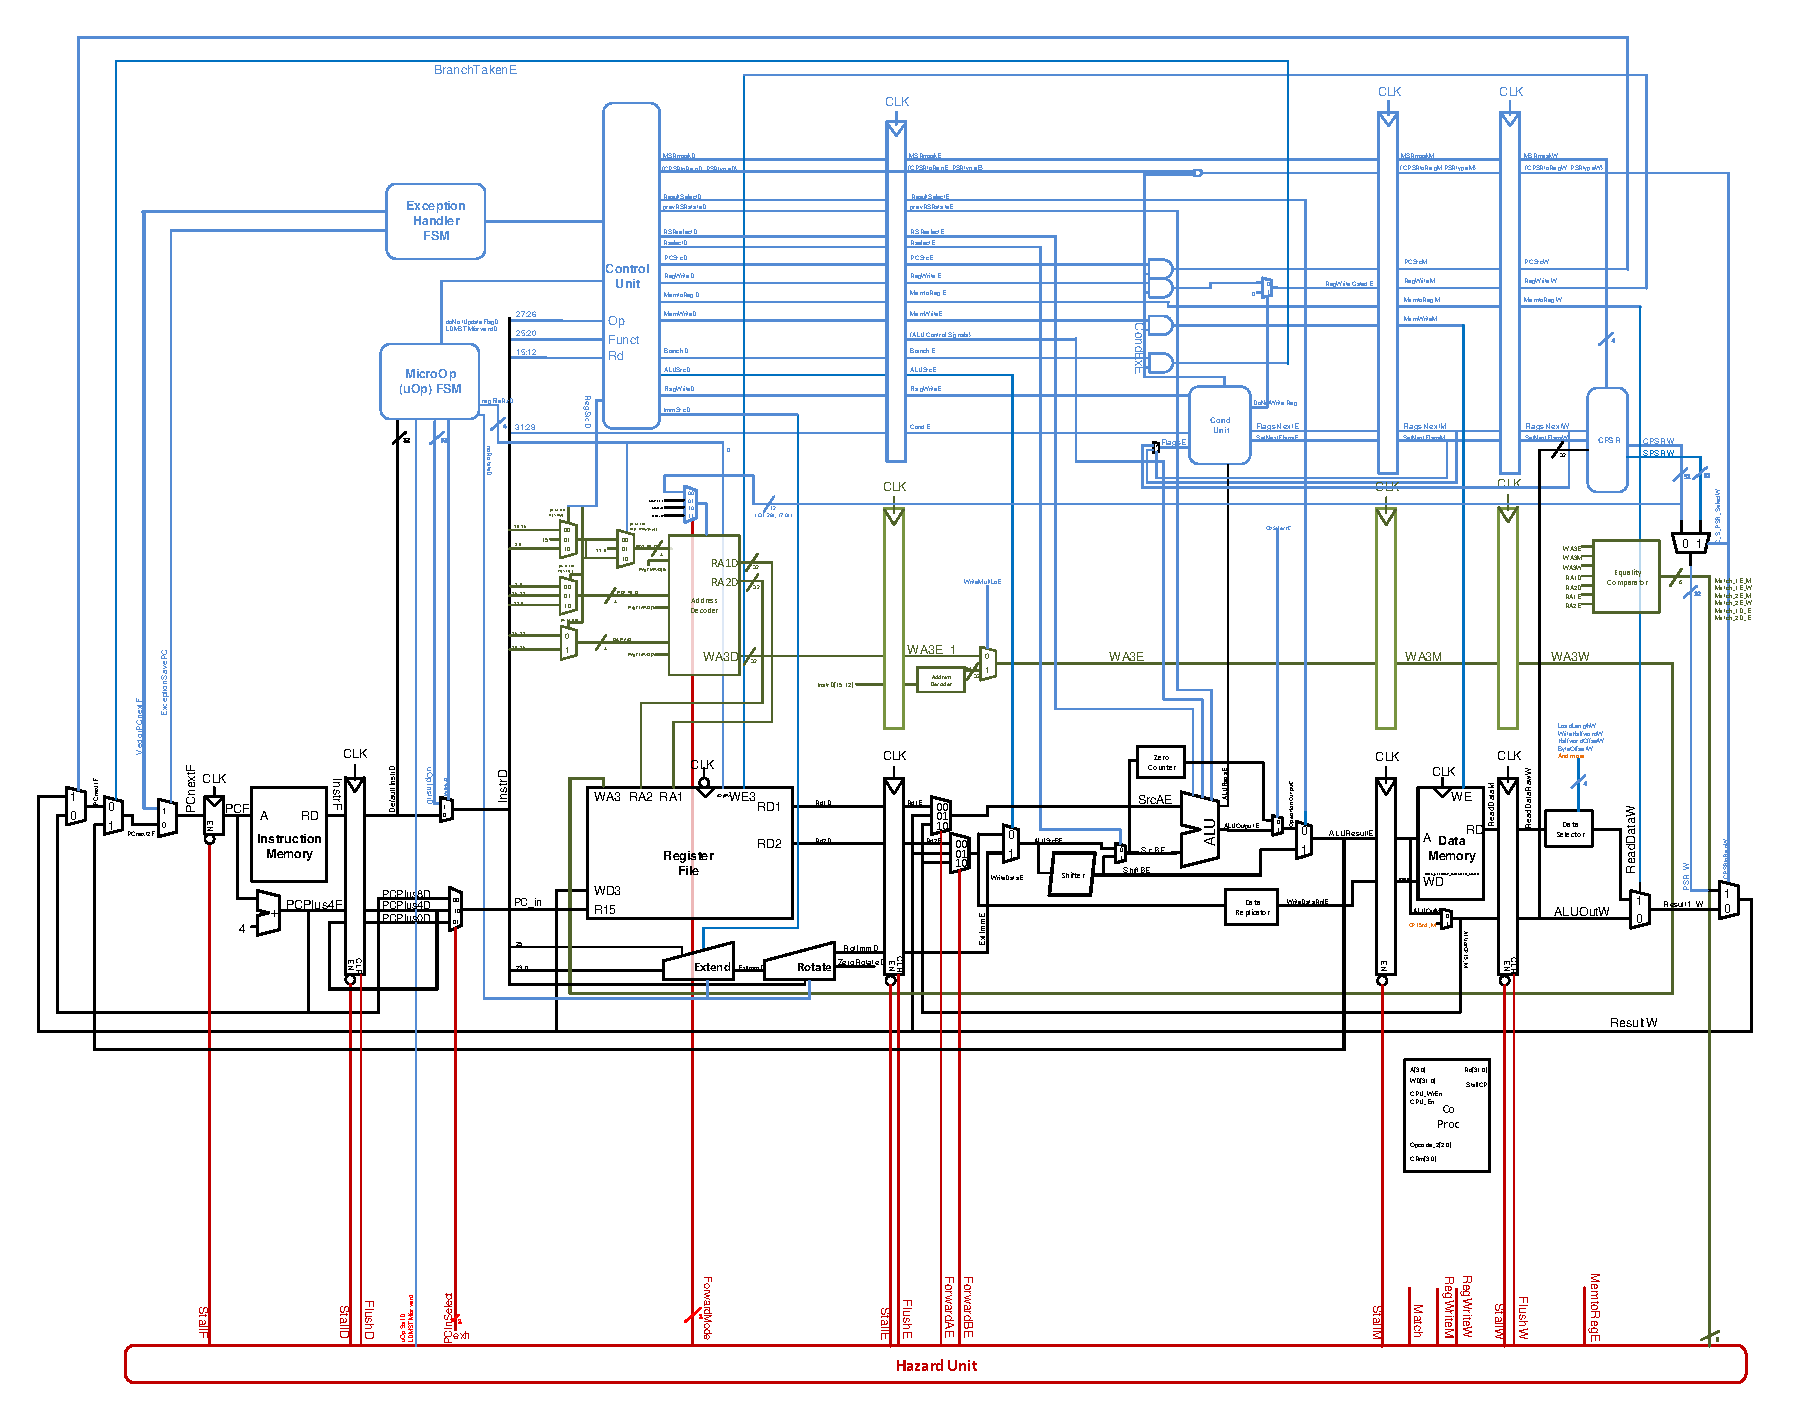
\includegraphics[width=\textwidth]{./diagrams/pipelinedfull.pdf}
\caption{LEG pipeline showing datapath (black), controller (blue), hazard unit (red), and a register file decoder also called the addresspath (green).}
\label{fig:pipelinedfull}
\end{figure}

\subsection{Memory System}

\subsection{Core and Memory Integration}

\subsection{Exception and Interrupt Handler}

The LEG interrupt handler supports all exception types and privileged modes with the Base Restored Abort Model.
The interrupt handler is implemented as a finite state machine in \texttt{leg\_pipelined/exception\_handler.sv}.
This state machine stalls the correct pipeline stages and controls the datapath to branch to the corresponding exception vector.
More information about the exception handler can be found in Section \ref{sec:exh}
